\documentclass[tikz,border=2pt]{standalone}
\usepackage{amsmath}
\usetikzlibrary{arrows.meta,decorations.pathreplacing}
\begin{document}
% A batch of B = 5 jobs of one colour: the k-th job waits for B-k further arrivals, i.e. 4,3,2,1,0
% inter-arrival times; the average over the batch is (B-1)/2 = 2 inter-arrival times, i.e. (B-1)/(2 lambda_i).
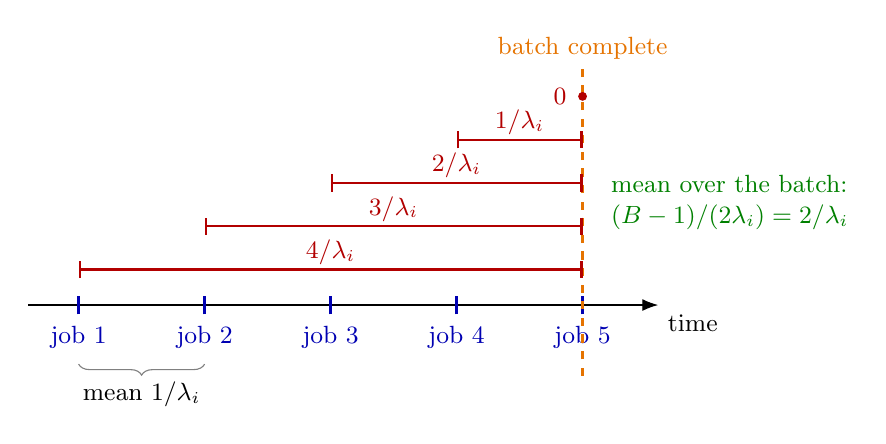
\begin{tikzpicture}[font=\small, >={Latex[length=2mm]}, x=1.6cm]
  \draw[->] (-0.4,0) -- (4.6,0) node[anchor=north west] {time};
  \foreach \k [count=\j] in {0,1,2,3,4} {
    \draw[blue!70!black, very thick] (\k,-0.12) -- (\k,0.12);
    \node[blue!70!black, anchor=north] at (\k,-0.15) {job $\j$};
  }
  \draw[orange!90!black, thick, dashed] (4,-0.9) -- (4,3.0);
  \node[orange!90!black, anchor=south] at (4,3.0) {batch complete};
  % waiting bars of each job until the batch is complete
  \foreach \k/\w in {0/4,1/3,2/2,3/1} {
    \draw[red!70!black, thick, |-|] (\k,0.45+0.55*\k) -- (4,0.45+0.55*\k);
    \node[red!70!black, anchor=south, fill=white, inner sep=1pt] at ({(\k+4)/2},0.47+0.55*\k) {$\w/\lambda_i$};
  }
  \fill[red!70!black] (4,2.65) circle (1.6pt);
  \node[red!70!black, anchor=east] at (3.95,2.65) {$0$};
  \draw[decorate, decoration={brace, amplitude=4pt, mirror}, gray] (0,-0.75) -- (1,-0.75)
    node[midway, below=3pt, black] {mean $1/\lambda_i$};
  \node[green!50!black, anchor=west, align=left] at (4.15,1.3) {mean over the batch:\\$(B-1)/(2\lambda_i)=2/\lambda_i$};
\end{tikzpicture}
\end{document}
